\documentclass{article}\usepackage[utf8]{inputenc}\usepackage[T1]{fontenc}\usepackage{lmodern}\usepackage{amsmath}\usepackage{tikz}\pagestyle{empty}\begin{document}\begin{center}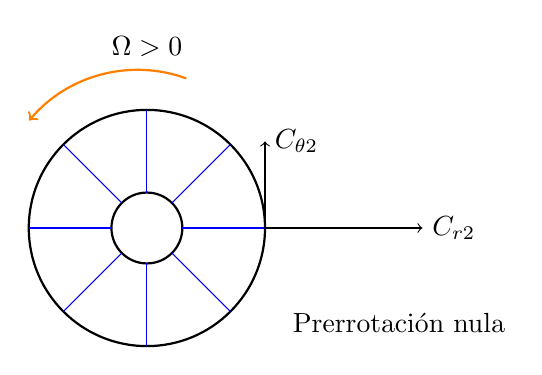
\begin{tikzpicture}\draw[thick] (2.5,1.7) circle (1.5);\draw[thick] (2.5,1.7) circle (.45);\foreach \a in {0,45,...,315}{\draw[blue,rotate around={\a:(2.5,1.7)}] (2.95,1.7)--(4,1.7);}\draw[->,orange,thick] (3,3.6) arc (70:140:1.8);\node at (2.5,4) {$\Omega>0$};\draw[->] (4,1.7)--(6,1.7) node[right] {$C_{r2}$};\draw[->] (4,1.7)--(4,2.8) node[right] {$C_{\theta2}$};\node at (5.7,.5) {Prerrotación nula};\end{tikzpicture}\end{center}\end{document}